% !TeX program = lualatex
\documentclass[]{article}

\usepackage{caption,subcaption,graphicx,float,url,amsmath,amssymb,amsthm,tocloft,cancel,thmtools,gensymb,braket,tikz-feynman,mathtools,color, colortbl}
\usepackage[toc,nonumberlist]{glossaries}
\usepackage{glossaries-extra}
\usepackage[toc,page]{appendix}

\newcommand\numberthis{\addtocounter{equation}{1}\tag{\theequation}}
\renewcommand{\thesection}{1.\arabic{section}}
\newtheorem{thm}{Theorem}
\newtheorem{defn}[thm]{Definition}
\newtheorem{cor}[thm]{Corollary}
\newtheorem{lemma}[thm]{Lemma}
\graphicspath{{figs/}}
\widowpenalty10000
\clubpenalty10000
\setcounter{tocdepth}{2}
\tikzfeynmanset{compat=1.1.0}
\definecolor{Gray}{gray}{0.5}
\DeclareMathOperator{\Tr}{Tr \;}
\newcommand{\Lagr}{\mathcal{L}}
\setlength{\cftsubsecindent}{0em}
\setlength{\cftsecnumwidth}{3em}
\setlength{\cftsubsecnumwidth}{3em}

%opening
\title{Quantum Field Theory\\
Part I: Motivation and Foundation}
\author{Simon Crase (compiler)\\simon@greenweaves.nz}



\begin{document}

\maketitle

\begin{abstract}

This document contains derivations of equations from \cite[Part I: Motivation and Foundation]{zee2010quantum}.

\end{abstract}

\tableofcontents


\section{Path Integral Formulation}

\begin{thm}[Some useful integrals]
	\begin{align*}
		\int_{-\infty}^{\infty} dx e^{-\frac{1}{2}x^2} =& \sqrt{2\pi} \numberthis \label{eq:integral:gaussian0}\\
		\int_{-\infty}^{\infty} dx e^{-\frac{1}{2}ax^2} =& \bigg(\frac{2\pi}{a}\bigg)^\frac{1}{2} \numberthis \label{eq:integral:gaussian}\\
		\int_{-\infty}^{\infty} dx\,e^{-\frac{a}{2} x^2+Jx}=&\bigg(\frac{2\pi}{a}\bigg)^\frac{1}{2}e^\frac{J^2}{2a} \numberthis \label{eq:integral:gaussian1}\\
		\int_{-\infty}^{\infty} dx\,e^{-\frac{a}{2} x^2+iJx}=&\bigg(\frac{2\pi}{a}\bigg)^\frac{1}{2}e^{-\frac{J^2}{2a}} \numberthis \label{eq:integral:gaussian2}
	\end{align*}
\end{thm}

\begin{proof}
	\begin{align*}
		\int_{-\infty}^{\infty} dx e^{-\frac{1}{2}x^2}\big)\big(\int_{-\infty}^{\infty} dy e^{-\frac{1}{2}y^2}\big) =& \int_{-\infty}^{\infty} \int_{-\infty}^{\infty} dx dy e^{-\frac{1}{2}(x^2+y^2)} \\
		=& \int_{0}^{2\pi} d\theta \int_{0}^{\infty}dr\;r\;e^\frac{-r^2}{2} \text{, substituting $x=r\cos{\theta}$,$y=r\sin{\theta}$}\\
		=&- 2\pi \int_{0}^{\infty}du e^{-u}\;\text{, substituting $u=\frac{-r^2}{2}$}\\
		=&- 2\pi e^{-u}\bigg\vert_0^\infty\\
		=& 2\pi
	\end{align*}
	Taking square roots of both side, we get \eqref{eq:integral:gaussian0}.
	\begin{align*}
		\int_{-\infty}^{\infty} dx e^{-\frac{1}{2}ax^2} =&\frac{1}{\sqrt{a}} \int_{-\infty}^{\infty} dx^\prime e^{-\frac{1}{2}{x^\prime}^2} \text{, substituting $x^\prime = \sqrt{a}x$} \\
		=& \bigg(\frac{2\pi}{a}\bigg)^\frac{1}{2} \text{, from \eqref{eq:integral:gaussian0}, 	which gives \eqref{eq:integral:gaussian}}
	\end{align*}

	\begin{align*}
		\int_{-\infty}^{\infty} dx\,e^{-\frac{a}{2} x^2+Jx}=&\int_{-\infty}^{\infty} dx\,e^{-\frac{a}{2} \big[x^2-2 \big(\frac{J}{a}\big)x+\big(\frac{J}{a}\big)^2\big]} e^{\frac{a}{2}\big(\frac{J}{a}\big)^2}\text{, completing the square}\\
		=&e^\frac{J^2}{2a}\int_{-\infty}^{\infty} dx e^{-\frac{a}{2} \big[x-\frac{J}{a}\big]^2} \text{, now substitute $x^\prime=x-\frac{J}{a}$}\\
		=&e^\frac{J^2}{2a}\int_{-\infty}^{\infty} dx^\prime e^{-\frac{a}{2} {x^\prime}^2}
	\end{align*}
	Substituting \eqref{eq:integral:gaussian} gives \eqref{eq:integral:gaussian1}. Replacing $J$ by $iJ$ gives \eqref{eq:integral:gaussian2}.
\end{proof}



\begin{thm}[Feynman Path Integral--Exercise I.2.1 - eq(5)]
	If the Hamiltonian is given by
	\begin{align*}
		H =& \frac{\hat{p}^2}{2m} + V(\hat{q}) \text{, and the corresponding Lagrangian is} \numberthis \label{eq:H} \\
		L =& \frac{\hat{p}^2}{2m} - V(\hat{q}) \text{, then} \numberthis \label{eq:L}\\
		\braket{q_F\vert H\vert q_I} =& \int Dq(t) e^{i \int_{0}^{T}dt L} \text{, where}\numberthis \label{eq:Path:itegral}\\	
		\int Dq(t)\triangleq& \lim_{N\rightarrow\infty} \big(\frac{-i m}{2\pi \delta t}\big)^\frac{N}{2} \big(\prod_{j=1}^{N-1} \int dq_j\big) \numberthis \label{eq:D}
	\end{align*}
\end{thm}
\begin{proof}
	For some N, define $\delta t =T/N$ and $q_j= q(j \delta t)$.
	
	\begin{align*}
		\braket{q_F\vert H\vert q_I} =& \big(\prod_{j=1}^{N-1} \int dq_j\big)\prod_{i=0}^{N-1} \braket{q_{j+1} \vert e^{-iHT} \vert q_j}\\
		=& \big(\prod_{j=1}^{N-1} \int dq_j\big)\prod_{i=0}^{N-1} \braket{q_{j+1} \vert e^{-i\big(\frac{\hat{p}^2}{2m} + V(\hat{q})\big)\delta t} \vert q_j} \text{, from \eqref{eq:H}}\\
		=& \big(\prod_{j=1}^{N-1} \int dq_j\big)\prod_{i=0}^{N-1} \braket{q_{j+1} \vert e^{-i\frac{\hat{p}^2}{2m} \delta t} e^{-i V(\hat{q}) \delta t} \vert q_j} \text{, we'll expand in eigenvectors of $\hat{q}$}\\
		=& \big(\prod_{j=1}^{N-1} \int dq_j\big)\prod_{i=0}^{N-1} \int dq \braket{q_{j+1} \vert e^{-i\frac{\hat{p}^2}{2m} \delta t}\vert q} \braket{q\vert e^{-i V(\hat{q}) \delta t} \vert q_j} \text{, since $\ket{q}\bra{q}=I$} \numberthis \label{eq:qHq}
	\end{align*}
	 We will evaluate the integrand in two steps, starting with the potential energy.
	\begin{align*}
		\braket{q\vert e^{-i V(\hat{q}) \delta t} \vert q_j} =& \braket{ e^{i V(\hat{q}) \delta t} q \vert q_j}\\
		=& \braket{ e^{i V(q) \delta t} q \vert q_j} \text{, since $\ket{q}$ is an eigenvector, with eigenvalue $q$}\\
		=& \braket{ e^{i V(q) \delta t} q \vert q_j} \\
		=& e^{-i V(q) \delta t} \braket{ q \vert q_j}  \numberthis \label{eq:qVq}
	\end{align*}
	Now for the kinetic energy.
	\begin{align*}
		\braket{q_{j+1} \vert e^{-i\frac{\hat{p}^2}{2m} \delta t}  \vert q}=& \int \frac{dp}{2\pi}\braket{q_{j+1} \vert e^{-i\frac{\hat{p}^2}{2m} \delta t}  \vert p} \braket{p\vert q}\\
		=& \int \frac{dp}{2\pi} e^{-i\frac{p^2}{2m} \delta t} \braket{q_{j+1} \vert p} \braket{p\vert q} \text{, since $\ket{p}$ is an eigenvector of $\hat{p}$}\\
		=& \int \frac{dp}{2\pi} e^{-i\frac{p^2}{2m} \delta t} e^{ip q_{j+1}} e^{-ip q} 
	\end{align*}
	Using \eqref{eq:integral:gaussian2} with $a=\frac{i \delta t}{m}$ and $J=q_{j+1}-q$:
	\begin{align*}
	\braket{q_{j+1} \vert e^{-i\frac{\hat{p}^2}{2m} \delta t}  \vert q}=& \int \frac{dp}{2\pi} e^{\frac{-i \delta t}{2m}p^2} e^{ip [q_{j+1}-q]} \\
	=& \frac{1}{2\pi} \big(\frac{2\pi m}{i \delta t}\big)^\frac{1}{2} e^{-\frac{m (q_{j+1}-q)^2}{2 i \delta t}}\\
	=& \big(\frac{-i m}{2\pi \delta t}\big)^\frac{1}{2} e^{i \delta t \frac{m (q_{j+1}-q)^2}{2  {\delta t}^2}}  \numberthis \label{eq:qP2q}
	\end{align*}
	Substituting \eqref{eq:qVq} and \eqref{eq:qP2q} in \eqref{eq:qHq}: 
	\begin{align*}
		\braket{q_F\vert H\vert q_I} =& \big(\frac{-i m}{2\pi \delta t}\big)^\frac{N}{2} \big(\prod_{j=1}^{N-1} \int dq_j\big) \prod_{i=0}^{N-1} \big(\frac{-i m}{2\pi \delta t}\big)^\frac{1}{2} \int dq e^{i \delta t \frac{m (q_{j+1}-q)^2}{2  {\delta t}^2}} e^{-i V(q) \delta t} \underbrace{\braket{ q \vert q_j}}_\text{$=m^2$}\delta(q-q_j) \\
		=& \big(\frac{-i m}{2\pi \delta t}\big)^\frac{N}{2} \big(\prod_{j=1}^{N-1} \int dq_j\big) \prod_{j=0}^{N-1}  e^{i \delta t \bigg[\frac{m (q_{j+1}-q_j)^2}{2  {\delta t}^2} - V(q_j)\bigg]}\\
		=& \big(\frac{-i m}{2\pi \delta t}\big)^\frac{N}{2} \big(\prod_{j=1}^{N-1} \int dq_j\big)  e^{i  \sum_{i=0}^{N-1} \delta t \bigg[\frac{m (q_{j+1}-q_j)^2}{2  {\delta t}^2} - V(q_j)\bigg]} \numberthis \label{eq:big:feynman:sum}
	\end{align*}
	Now, as $N\rightarrow\infty$
	\begin{align*}
	\sum_{i=0}^{N-1} \delta t \rightarrow &\int dt\\
	\frac{m (q_{j+1}-q_j)^2}{2  {\delta t}^2} \rightarrow & \frac{m \dot{q}}{2} \text{, so, substituting \eqref{eq:L} and \eqref{eq:D}, \eqref{eq:big:feynman:sum} becomes}\\
	\braket{q_F\vert H\vert q_I} \rightarrow& \int Dq(t) e^{i \int_{0}^{T}dt L} \text{i.e. \eqref{eq:Path:itegral}}
	\end{align*}
\end{proof}




\begin{thm}
	\begin{align*}
		\frac{\int_{-\infty}^\infty dx e^{-\frac{1}{2}ax^2}x^{2n}}{\int_{-\infty}^\infty dx e^{-\frac{1}{2}ax^2}} =&\frac{\prod_{k=1}^{n}\big(2k-1\big)}{a^n}
	\end{align*}
\end{thm}

\begin{proof}
	The proof by mathematical induction starts by defining the proposition $P(n)$:
	\begin{align*}
		P(n) \equiv& \bigg[\frac{\int_{-\infty}^\infty dx e^{-\frac{1}{2}ax^2}x^{2n}}{\int_{-\infty}^\infty dx e^{-\frac{1}{2}ax^2}}=\frac{\prod_{k=1}^{n}\big(2k-1\big)}{a^n}\bigg]
	\end{align*}
	\begin{lemma}\label{thm:P_0}
		P(0) is true.
	\end{lemma}
	\begin{proof}
		$P(0)$ reduces to $\frac{\int_{-\infty}^\infty dx e^{-\frac{1}{2}ax^2}}{\int_{-\infty}^\infty dx e^{-\frac{1}{2}ax^2}}=1$
	\end{proof}
    \begin{lemma}\label{lemma:uniform:convergence}
    	\begin{align*}
    		\forall \alpha >0 \text{, }\frac{d}{d\alpha}\int_{-\infty}^\infty dx e^{-\frac{1}{2}\alpha x^2}x^{2n} =&\int_{-\infty}^\infty dx \frac{\partial}{\partial \alpha} \big[e^{-\frac{1}{2}\alpha x^2}x^{2n}\big]
    	\end{align*}
    \end{lemma}
	\begin{proof}
		\begin{align*}
			\forall a>0, \forall \alpha_0 \in (0,\alpha)\; \int_{a}^\infty dx e^{-\frac{1}{2}\alpha x^2}x^{2n} =&\int_{a}^\infty dx e^{-\frac{1}{2}\alpha_0 x^2} e^{-\frac{1}{2}(\alpha-\alpha_0) x^2}x^{2n} \\
			\text{Now define}\; M(x) =& e^{-\frac{1}{2}\alpha_0 x^2}
		\end{align*}
		We can choose $a$ large enough that $e^{-\frac{1}{2}(\alpha-\alpha_0) x^2}x^{2n}$ is monotone decreasing for $x>a$. Clearly
		\begin{align*}
			e^{-\frac{1}{2}\alpha_0 x^2} e^{-\frac{1}{2}(\alpha-\alpha_0) x^2}x^{2n} \in C\\
				e^{-\frac{1}{2}\alpha_0 x^2} \in C\\
			e^{-\frac{1}{2}\alpha_0 x^2} e^{-\frac{1}{2}(\alpha-\alpha_0) x^2}x^{2n}<&M(x)\; \forall x>a \text{ and}\\
			\int_{a}^\infty dx M(x)<&\infty
		\end{align*}
		 for $\alpha$ in closed interval [A,B] that includes $\alpha_0$; the Weierstrass M-Test \cite[Chapter 10, 6.1]{widder1961advanced} shows that the integral converges uniformly for $\alpha\in[A,B]$. Hence we can differentiate under the integral sign \cite[Chapter 10, 8.3]{widder1961advanced}.
		Now
		\begin{align*}
			\int_{-\infty}^\infty dx e^{-\frac{1}{2}\alpha x^2}x^{2n} =& 2 \int_{a}^\infty dx e^{-\frac{1}{2}\alpha x^2}x^{2n} + \int_{-a}^a dx e^{-\frac{1}{2}\alpha x^2}x^{2n}
		\end{align*}
	Noting that $e^{-\frac{1}{2}\alpha x^2}x^{2n} \in C^1$ for x in [-a,a], we can also differentiate the second integral.
	\end{proof}

	\begin{lemma}\label{thm:P_1}
		$P(0) \implies P(1)$
	\end{lemma}
	\begin{proof}
		Since (\ref{eq:integral:gaussian}) converges uniformly, Lemma \ref{lemma:uniform:convergence} allows us to differentiate under the integral sign\cite{widder1961advanced}.
		\begin{align*}
			-2\frac{d}{da}\int_{-\infty}^{\infty} dx e^{-\frac{1}{2}ax^2} =& -2\frac{d}{da} \bigg(\frac{2\pi}{a}\bigg)^\frac{1}{2}\\
			\int_{-\infty}^{\infty} dx e^{-\frac{1}{2}ax^2} x^2 =& \bigg(\frac{2\pi}{a^3}\bigg)^\frac{1}{2}\\
			=& \bigg(\frac{2\pi}{a}\bigg)^\frac{1}{2} \frac{1}{a}\\
			=& \int_{-\infty}^{\infty} dx e^{-\frac{1}{2}ax^2} \frac{1}{a}
		\end{align*}
	\end{proof}
	\begin{lemma}\label{thm:P_n}
		$P(n) \land P(1)\implies P(n+1)$
	\end{lemma}
	\begin{proof}
		\begin{align*}
		P(n) \implies &\\
		\int_{-\infty}^\infty dx e^{-\frac{1}{2}ax^2}x^{2n}=&\prod_{k=1}^{n}\big(2k-1\big)	\int_{-\infty}^\infty dx e^{-\frac{1}{2}ax^2} \frac{1}{a^n}\\
		-2\frac{d}{da}\int_{-\infty}^\infty dx e^{-\frac{1}{2}ax^2}x^{2n}=&-2 \prod_{k=1}^{n}\big(2k-1\big)\frac{d}{da} \big[	\int_{-\infty}^\infty dx e^{-\frac{1}{2}ax^2} \frac{1}{a^n}\big]\\
		\int_{-\infty}^\infty dx e^{-\frac{1}{2}ax^2}x^{2(n+1)}=&-2 \prod_{k=1}^{n}\big(2k-1\big)\bigg[\int_{-\infty}^{\infty} dx e^{-\frac{1}{2}ax^2} (-\frac{1}{2}x^2)\frac{1}{a^n}-\int_{-\infty}^{\infty} dx e^{-\frac{1}{2}ax^2}\frac{n}{a^{n+1}}\bigg] \\
		=&\prod_{k=1}^{n}\big(2k-1\big)\bigg[\underbrace{\int_{-\infty}^{\infty} dx e^{-\frac{1}{2}ax^2}x^2}_\text{Now we apply $P(1)$} \frac{1}{a^n}+2\int_{-\infty}^{\infty} dx e^{-\frac{1}{2}ax^2}\frac{n}{a^{n+1}}\bigg]\\
		=&\prod_{k=1}^{n}\big(2k-1\big)\bigg[ \int_{-\infty}^{\infty} dx e^{-\frac{1}{2}ax^2}\frac{1}{a} \frac{1}{a^n} + \int_{-\infty}^{\infty} dx e^{-\frac{1}{2}ax^2} \frac{2n}{a^{n+1}}\bigg]\\
		=&\prod_{k=1}^{n}\big(2k-1\big) \frac{2n+1}{a^{n+1}}\int_{-\infty}^{\infty} dx e^{-\frac{1}{2}ax^2}\\
		=&\prod_{k=1}^{n+1}\big(2k-1\big) \frac{1}{a^{n+1}}\int_{-\infty}^{\infty} dx e^{-\frac{1}{2}ax^2}\\
		\equiv& P(n+1)
		\end{align*}
	\end{proof}
	Summarizing:
	\begin{align*}
		\text{Lemma }\ref{thm:P_0} \implies& P(0)\\
		P(0) \land \text{Lemma } \ref{thm:P_1} \implies& P(1)\\
		P(0) \land P(1)\land P(n) \land \text{Lemma } \ref{thm:P_n} \implies& P(n+1)
	\end{align*}
\end{proof}

\begin{thm}
	If $A$ is a symmetric matrix
	\begin{align*}
		\int_{-\infty}^{\infty}dx_1 dx_2...dx_N e^{-\frac{1}{2}\vec{x}A\vec{x} + \vec{J} \cdot \vec{x}} =& \bigg(\frac{(2\pi)^N}{\vert A \vert}\bigg)^\frac{1}{2} e^{\frac{1}{2}\vec{J}\cdot A^{-1} \vec{J}} \numberthis \label {eq:Zee_I_2_22}
	\end{align*}
\end{thm}
\begin{proof}
	Since $A$ is symmetric, there exists an orthogonal matrix $O$ such that $A=O^T D O$, where $D$ is a diagonal matrix--\cite{bellman1970introduction}. Define
	\begin{align*}
		y_i =& \sum_j O_{ij}x_j\\
		\int_{-\infty}^{\infty}dx_1 dx_2...dx_N e^{-\frac{1}{2}\vec{x}A\vec{x} + \vec{J} \cdot \vec{x}}=&\bigg(\frac{1}{\vert O \vert}\bigg)^N \int_{-\infty}^{\infty}dy_1 dy_2...dy_Ne^{-\frac{1}{2}\vec{x}O^T D O\vec{x} + \vec{J} \cdot \vec{x}}\\
		=& \int_{-\infty}^{\infty}dy_1 dy_2...dy_N e^{-\frac{1}{2}(\vec{x}O^T) D (O\vec{x}) + \vec{J} \cdot \vec{x}}\\
		=& \int_{-\infty}^{\infty}dy_1 dy_2...dy_N e^{- \frac{1}{2} \vec{y}D \vec{y} + (O\vec{J})\cdot \vec{y}}\\
		=& \prod_{i=1}^N \int_{-\infty}^{\infty}dy_i e^{- \frac{1}{2} D_{ii}y_i^2 + (OJ)_i y_i}\\
		=& \prod_{i=1}^N \bigg[\bigg(\frac{2\pi}{D_{ii}}\bigg)^\frac{1}{2} e^{\big(\frac{[(OJ)_i]^2}{2D_{ii}}\big)}\bigg] \numberthis \label {eq:Zee_I_2_22_a}
	\end{align*}
	But
	\begin{align*}
		\prod_{i=1}^N \bigg(\frac{2\pi}{D_{ii}}\bigg) =& \frac{({2\pi})^N}{\vert D \vert}\\
		=& \frac{({2\pi})^N}{\vert A \vert} \text{, since $O$ is orthogonal} \numberthis \label {eq:Zee_I_2_22_b}
	\end{align*}
	And
	\begin{align*}
		\prod_{i=1}^N e^{\big(\frac{[(OJ)_i]^2}{2D_{ii}}\big)} =& e^{\sum_{i=1}^N {\big(\frac{[(OJ)_i]^2}{2D_{ii}}\big)}}\\
		\sum_{i=1}^N {\big(\frac{[(OJ)_i]^2}{2D_{ii}}\big)} =& \frac{1}{2} \sum_{i=1}^N (OJ)_i (D^{-1})_{ii} (OJ)_i\\
		 =& \frac{1}{2} \sum_{i,j,k,l=1}^N O_{ik} J_k (D^{-1})_{ij} O_{jl} J_l\\
		 =& \frac{1}{2} \sum_{i,j,k,l=1}^N J_k O^T_{ki}  (D^{-1})_{ij} O_{jl} J_l \\
		 =& \frac{1}{2} \sum_{k,l=1}^N J_k \bigg(\sum_{k,l=1}^N O^T_{ki}  (D^{-1})_{ij} O_{jl}\bigg) J_l\\
		  \\
		 =& \frac{1}{2} \sum_{k,l=1}^N J_k \big(A^{-1}\big)_{kl} J_l \\
		 =& \frac{1}{2} J A^{-1} J \numberthis \label {eq:Zee_I_2_22_c}
	\end{align*}
	Substituting (\ref{eq:Zee_I_2_22_b}) and (\ref{eq:Zee_I_2_22_c}) in (\ref{eq:Zee_I_2_22_a}), we obtain (\ref{eq:Zee_I_2_22}).
\end{proof}

\section{From Field to Particle to Force}
\begin{align*}
	W(J) =& - \frac{1}{2} \int \int d^4x d^4y J(x) D(x-y) J(y)\\
	D(x-y) =& \int \frac{d^4k}{(2\pi)^4} \frac{e^{ik(x-y)}}{k^2-m^2+i\epsilon}\\
	J(x) =& J_1(x) + J_2(x) \text{, where}\\
	J_{a}(x) =&\delta^{(3)}(\vec{x}-\vec{x_a}) 
\end{align*}
Considering only the cross terms
\begin{align*}
	W(J) =& - \int \frac{1}{(2\pi)^4} \cancel{2} \cancel{\frac{1}{2}} \int \int d^4x d^4y d^4k \delta^{(3)}(\vec{x}-\vec{x_1})   \frac{e^{ik(x-y)}}{k^2-m^2+i\epsilon} \delta^{(3)}(\vec{y}-\vec{x_2}))\\
	=& - \frac{1}{(2\pi)^4} \int \int \int \int \int \int dx^0 d\vec{x} dy^0 d\vec{y} dk^0 d\vec{k}  \delta^{(3)}(\vec{x}-\vec{x_1})   \frac{e^{ik^0(x^0-y^0)-i\vec{k} \cdot (\vec{x}-\vec{y})}}{k^2-m^2+i\epsilon} \delta^{(3)}(\vec{y}-\vec{x_2}))\\
	=& - \frac{1}{(2\pi)^4} \int \int \int \int \int dx^0 d\vec{x} dy^0 dk^0 d\vec{k}  \delta^{(3)}(\vec{x}-\vec{x_1})   \frac{e^{ik^0(x^0-y^0)-i\vec{k} \cdot (\vec{x}-\vec{x_2})}}{k^2-m^2+i\epsilon} \\
	=& - \frac{1}{(2\pi)^4} \int \int \int \int dx^0  dy^0 dk^0 d\vec{k} \;    \frac{e^{ik^0(x^0-y^0)-i\vec{k} \cdot (\vec{x_1}-\vec{x_2})}}{k^2-m^2+i\epsilon}\\
	=& - \frac{1}{(2\pi)^3} \int \int dx^0  dy^0 \underbrace{\int \frac{dk^0}{2\pi} e^{ik^0(x^0-y^0)}}_\text{$\delta(x^0-y^0)$} \int d\vec{k} \; \frac{e^{i\vec{k} \cdot (\vec{x}-\vec{y})}}{k^2-m^2+i\epsilon}\\
	=& - \frac{1}{(2\pi)^3} \int  dx^0  \int d\vec{k} \; \frac{e^{i\vec{k} \cdot (\vec{x}-\vec{y})}}{k^2-m^2+i\epsilon}
\end{align*}

\section{Coulomb and Newton}
The Lagrangian Density is given by:
\begin{align*}
	\Lagr =& -\frac{1}{4} F_{\mu\nu}F^{\mu\nu} + \frac{1}{2}m^2 A_{\mu}A^{\mu} + A_{\mu}J^{\mu} \text{, where}\\
	F_{\mu\nu} =& \partial_{\mu} A_{\nu} - \partial_{\nu} A_{\mu} \text{ and}\\
	\partial_{\mu}J^{\nu}=& 0 \text{. We define the action} \numberthis \label{eq:EM_continuity}\\
	S(A) =&\int d^4 \Lagr\\
	=&  \int d^4x \bigg[-\frac{1}{4} F_{\mu\nu}F^{\mu\nu} + \frac{1}{2}m^2 A_{\mu}A^{\mu} + A_{\mu}J^{\mu} \bigg]
\end{align*}
Expanding the first term in the Lagrangian
\begin{align*}
	F_{\mu\nu}F^{\mu\nu}=& g^{\mu\rho} g^{\nu\sigma}F_{\mu\nu}F_{\rho\sigma}\\
	=& g^{\mu\rho} g^{\nu\sigma} \big(\partial_{\mu} A_{\nu} - \partial_{\nu} A_{\mu}\big)\big(\partial_{\rho} A_{\sigma} - \partial_{\sigma} A_{\rho}\big)\\
	=& g^{\mu\rho} g^{\nu\sigma}\big[\partial_{\mu} A_{\nu}\partial_{\rho} A_{\sigma} -\partial_{\mu} A_{\nu}\partial_{\sigma} A_{\rho} -\partial_{\nu} A_{\mu}\partial_{\rho} A_{\sigma} + \partial_{\nu} A_{\mu}\partial_{\sigma} A_{\rho}\big]\\
	=& g^{\mu\rho} g^{\nu\sigma} \partial_{\mu} A_{\nu}\partial_{\rho} A_{\sigma} -g^{\mu\rho} g^{\nu\sigma} \partial_{\mu} A_{\nu}\partial_{\sigma} A_{\rho} -\underbrace{g^{\mu\rho} g^{\nu\sigma} \partial_{\nu} A_{\mu}\partial_{\rho} A_{\sigma}}_\text{substitute: $\mu\nu\rho\sigma\rightarrow\nu\mu\sigma\rho$} +\underbrace{g^{\mu\rho} g^{\nu\sigma} \partial_{\nu} A_{\mu}\partial_{\sigma} A_{\rho}}_\text{$\mu\nu\rho\sigma\rightarrow\nu\mu\sigma\rho$}	\\
	=& g^{\mu\rho} g^{\nu\sigma} \partial_{\mu} A_{\nu}\partial_{\rho} A_{\sigma} -g^{\mu\rho} g^{\nu\sigma} \partial_{\mu} A_{\nu}\partial_{\sigma} A_{\rho} - g^{\nu\sigma} g^{\mu\rho} \partial_{\mu} A_{\nu}\partial_{\sigma} A_{\rho} +g^{\nu\sigma} g^{\mu\rho} \partial_{\mu} A_{\nu}\partial_{\rho} A_{ssigma}	\\
	=& 2 \big[g^{\mu\rho} g^{\nu\sigma} \partial_{\mu} A_{\nu}\partial_{\rho} A_{\sigma} -g^{\mu\rho} g^{\nu\sigma} \partial_{\mu} A_{\nu}\partial_{\sigma} A_{\rho}\big]
\end{align*}
So the first term in the action is
\begin{align*}
	 -\frac{1}{4} \int d^4x F_{\mu\nu}F^{\mu\nu} =&  -\frac{2}{4} \int d^4x \big[g^{\mu\rho} g^{\nu\sigma} \partial_{\mu} A_{\nu}\partial_{\rho} A_{\sigma} -g^{\mu\rho} g^{\nu\sigma} \partial_{\mu} A_{\nu}\partial_{\sigma} A_{\rho}\big] \text{. Integrating by parts gives}\\
	 =& \frac{1}{2} \int d^4x \big[g^{\mu\rho} g^{\nu\sigma}  A_{\nu}\partial_{\mu}\partial_{\rho} A_{\sigma} -g^{\mu\rho} g^{\nu\sigma}  A_{\nu}\partial_{\mu} \partial_{\sigma} A_{\rho}\big]\\
	 =& \frac{1}{2} \int d^4x \big[ g^{\nu\sigma}  A_{\nu}\partial^2 A_{\sigma} -  A_{\nu}\partial^{\rho} \partial^{\nu} A_{\rho}\big]\\
	 =& \frac{1}{2} \int d^4x A_{\nu} \big[ g^{\nu\sigma}  \partial^2  -  \partial^{\sigma} \partial^{\nu} \big] A_{\sigma}
\end{align*}

So the action becomes
\begin{align*}
	\int d^4 \Lagr=&  \int d^4x \bigg[\frac{1}{2} A_{\nu} \big[ g^{\nu\sigma}  \partial^2  -  \partial^{\sigma} \partial^{\nu} \big] A_{\sigma} + \frac{1}{2}m^2 A_{\mu}A^{\mu} + A_{\mu}J^{\mu} \bigg]\\
	=&\int d^4x \bigg[\frac{1}{2} A_{\nu} \big[ g^{\nu\sigma}  (\partial^2 +m^2)  -  \partial^{\sigma} \partial^{\nu} \big] A_{\sigma} +  A_{\mu}J^{\mu} \bigg]
\end{align*}

\begin{align*}
	D_{\mu\nu} \big(D^{-1}\big)^{\nu\lambda} =& \delta_{\mu}^{\lambda}
\end{align*}
From Lecture. How do we get a repulsive force? This is tied up with spin. If we want particles fro field to have spin 1, we need a vector--$A_{\mu}$. We need to reduce $A_{\mu}$ to 3 degrees of freedom (polarization), and \eqref{eq:EM_continuity} is the only Lorentz invariant way to do this. We will start with the physics--Figure \ref{fig:electromagnetic:current}.
\begin{figure}[H]
	\begin{center}
		\caption{Electromagnetic Field with source and sink}\label{fig:electromagnetic:current}
		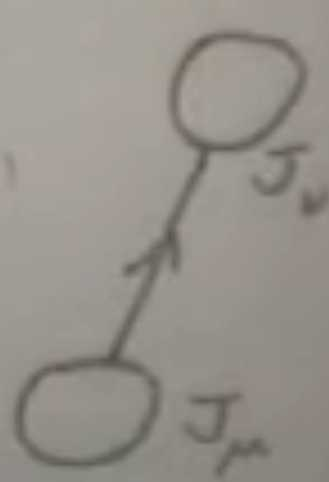
\includegraphics[width=0.5\textwidth]{qft_liecture2_1}
	\end{center}
\end{figure}
\begin{align*}
	J \phi \rightarrow& J_{\mu} A^{\mu}\\
	\frac{1}{k^2 + m^2} \rightarrow& \frac{1}{k^2 + m^2} \underbrace{\underbrace{\sum_{a=1}^{3}}_\text{3 polarizations} \epsilon_\mu^{(a)}(k) \epsilon_\nu^{(a)}(k)}_\text{A Lorentz tensor, $-G_{\mu\nu}$ say} \numberthis \label{eq:em:propagator}
\end{align*}
We will evaluate in the rest frame of the particle, where $k=(m,0,0,0)$, and polarization is the 3 directions in Cartesian space.
\begin{align*}
	\epsilon_\mu^{(1)}(k) =& (0,1,0,0)\\
	\epsilon_\mu^{(2)}(k) =& (0,0,1,0)\\
	\epsilon_\mu^{(3)}(k) =& (0,0,0,1)\\
	k^{\mu}\epsilon_\mu =& 0 \text{, since $k=(m,0,0,0)$} \numberthis \label{eq:k_mu_0}
\end{align*}
\eqref{eq:k_mu_0} is Lorentz Invariant! c.f. $\partial_{\mu}A^{\mu}=0$. We will establish the tensor $G_{\mu\nu}$ in \eqref{eq:em:propagator} using symmetry and Lorentz invariance. There are only two things to construct $G_{\mu\nu}$ from, $k_{\mu}$ and $g_{\mu\nu}$.
\begin{align*}
	- G_{\mu\nu} =& A k_{\mu} k_{\nu} + B g_{\mu\nu}\\
	 G_{\mu\nu} k^{\mu} =& 0 \text{ from \eqref{eq:k_mu_0}, whence}\\
	 \big(A k_{\mu} k_{\nu} + B g_{\mu\nu}\big) k^{\mu} =& 0\\
	 \big(A \underbrace{k^2}_\text{$=m^2$}+B\big)k_{\nu} =& 0\\
	 A =& -\frac{B}{m^2}\\
	 - G_{\mu\nu} =& -\big(g_{\mu\nu}-\frac{k_{\mu}k_{\nu}}{m^2}\big) \text{. Normalization fixed by rest frame.}\\
	 \frac{1}{k^2 + m^2} \rightarrow& \frac{-g_{\mu\nu}+\frac{k_{\mu}k_{\nu}}{m^2}}{k^2 + m^2}
\end{align*}
Imagine two stationary charges: then $J^i=0$
\begin{align*}
	W(J) =& \int  \frac{d^4k}{(2\pi)4} J^{\mu}(k)^* \frac{-g_{\mu\nu}+\frac{k_{\mu}k_{\nu}}{m^2}}{k^2 + m^2} J^{\nu}(k)\\
	\partial_{\mu} J^{\mu} =& 0 \text{ implies}\\
	k_{\mu} J^{\mu} =& 0\\
	W(J) =& \int  \frac{d^4k}{(2\pi)4} J^0(k)^* \frac{-g_{00}}{k^2 + m^2} J^0(k)\\
	=& \int  \frac{d^4k}{(2\pi)4} J^0(k)^* \frac{-1}{k^2 + m^2} J^0(k) \text{--Like charges repel}
\end{align*}

Spin 2 has two indices $h_{\mu\nu}$. Two sign switches cancel!

Even spin can exchange lumps, but not odd.

\begin{thm}
	\begin{align*}
		\big(\delta^2+m^2\big) A^{\mu}=&0 \text{ and} \numberthis \label{eq:cn:1}\\
		 \partial_{\mu} A^{\mu}=&0 \text{ are equivalent to } \numberthis \label{eq:cn:2}\\
		 \big(g^{\mu\nu}\partial^2-\partial^\mu\partial^\nu\big)A_\nu + m^2 A^\mu=&0 \numberthis \label{eq:cn:3}
	\end{align*}
\end{thm}
\begin{proof}[Proof: $\eqref{eq:cn:1} \land \eqref{eq:cn:2} \implies \eqref{eq:cn:3}$]
	 From	\eqref{eq:cn:2} 
	\begin{align*}
		 \partial^\nu A_\nu =& 0 \text{, whence}\\
		 \partial^\mu \partial^\nu A_\nu =& 0 \text{. Now \eqref{eq:cn:1} can be rearranged} \numberthis \label{eq:cn:4}\\
		 \partial^2 \big(g^{\mu\nu}A_\nu\big) + m^2 A^\mu =&0\\
		 g^{\mu\nu} \partial^2 A_\nu + m^2 A^\mu =&0 \text{. Now, using \eqref{eq:cn:4}}\\
		 g^{\mu\nu} \partial^2 A_\nu - \partial^\mu \partial^\nu A_\nu + m^2 A^\mu =&0 \text{, which rearranges to \eqref{eq:cn:3}}
	\end{align*}
\end{proof}
\begin{proof}[$\eqref{eq:cn:3} \implies \eqref{eq:cn:1} \land \eqref{eq:cn:2}$]
	From \eqref{eq:cn:3}
	\begin{align*}
	 	m^2 A^\mu=&\big(\partial^\mu\partial^\nu-g^{\mu\nu}\partial^2\big)A_\nu \\
	 	m^2 \partial_\mu A^\mu =&\partial_\mu \big(\partial^\mu\partial^\nu-g^{\mu\nu}\partial^2\big)A_\nu\\
	 	=&\partial_\mu\partial^\mu\partial^\nu A_\nu -  g^{\mu\nu}\partial_\mu\partial^2A_\nu\\
	 	=&\partial^2\partial^\nu A_\nu - \partial^\nu\partial^2A_\nu\\
	 	=& 0 \text{, which is \eqref{eq:cn:2}. Now \eqref{eq:cn:3} becomes}\\
	 	g^{\mu\nu}\partial^2 A_\nu-\cancel{\partial^\mu\partial^\nu A_\nu} + m^2 A^\mu=&0 \text{, which is \eqref{eq:cn:1}}
	\end{align*}
\end{proof}

\section{Feynman Diagrams}

\begin{align*}
	Z(J,\lambda) =& \int D\phi \; e^{i\int d^4x\;\big[\frac{1}{2}[(\partial \phi)^2-m^2\phi^2]-\frac{\lambda}{4!}\phi^4+J\phi\big]}\\
	=& \int D\phi \; e^{i\int d^4x\;\big[\frac{1}{2}[(\partial \phi)^2-m^2\phi^2]+J\phi\big]e^{-i\frac{\lambda}{4!}\phi^4}}
\end{align*}

The \emph{functional derivative} is defined in \cite{enwiki:1034704989}:
\begin{align*}
	\int \frac{\delta F(x)}{\delta \rho} \phi(x) dx \triangleq& \lim_{\epsilon \rightarrow 0} \frac{F(\rho + \epsilon \phi)-f[\rho]}{\epsilon}\\
	=&\bigg[\frac{dF(\rho+\epsilon\phi)}{d\rho}\bigg]_\text{$\epsilon=0$}
\end{align*}


\begin{thm}
	\begin{align*}
		Z(J,\lambda) =&	e^{-\frac{i\lambda}{4!}\int dx \frac{\delta^4}{(\delta J)^4}}Z(J,0)
	\end{align*}
\end{thm}

\begin{proof}
	After \cite{straub2004feynman}...	
\end{proof}


% Endmatter

\bibliographystyle{unsrt}
\addcontentsline{toc}{section}{Bibliography}
\raggedright
\bibliography{tm}

\end{document}
